%----------------------------------------------------------------------------------------
% PACKAGES AND DOCUMENT CONFIGURATIONS
%----------------------------------------------------------------------------------------

  \documentclass{article}

  \usepackage{hyperref}
  \usepackage{fancyhdr} % Required for custom headers
  \usepackage{lastpage} % Required to determine the last page for the footer
  \usepackage{extramarks} % Required for headers and footers
  \usepackage[usenames,dvipsnames]{color} % Required for custom colors
  \usepackage{graphicx} % Required to insert images
  \usepackage{listings} % Required for insertion of code
  \usepackage{courier} % Required for the courier font
  \usepackage{lipsum} % Used for inserting dummy 'Lorem ipsum' text into the template
  \usepackage{wrapfig}
  \usepackage{color}
  \usepackage{lscape}

  \setlength\parindent{0pt} % Removes all indentation from paragraphs
  \renewcommand{\labelenumi}{\alph{enumi}.} % Make numbering in the itemize environment by letter rather than number (e.g. section 6)

  % Margins
  \topmargin=-0.7in
  \evensidemargin=0.2in
  \oddsidemargin=-0.2in
  \textwidth=7.0in
  \textheight=9.3in
  % \headsep=0.25in

  % \linespread{1.1} % Line spacing

  \definecolor{dkgreen}{rgb}{0,0.6,0}
  \definecolor{gray}{rgb}{0.5,0.5,0.5}
  \definecolor{mauve}{rgb}{0.58,0,0.82}
  \definecolor{greyish}{rgb}{0.96,0.96,0.96}

  \lstset{
    backgroundcolor=\color{greyish},   % choose the background color; you must add \usepackage{color} or \usepackage{xcolor}
    frame=tb,
    numbers=left,                    % where to put the line-numbers; possible values are (none, left, right)
    numbersep=5pt,                   % how far the line-numbers are from the code
    numberstyle=\tiny\color{mygray}, % the style that is used for the line-numbers
    language=Ruby,
    aboveskip=3mm,
    belowskip=3mm,
    showstringspaces=false,
    columns=flexible,
    basicstyle={\footnotesize\ttfamily},
    numbers=none,
    numberstyle=\tiny\color{gray},
    keywordstyle=\color{blue},
    commentstyle=\color{dkgreen},
    stringstyle=\color{mauve},
    breaklines=true,
    breakatwhitespace=true
    tabsize=3
  }
%----------------------------------------------------------------------------------------
% DOCUMENT INFORMATION
%----------------------------------------------------------------------------------------
  \begin{document}
  \begin{titlepage}

%----------------------------------------------------------------------------------------
% TITLE PAGE INFORMATION
%----------------------------------------------------------------------------------------
 \newcommand{\HRule}{\rule{\linewidth}{0.5mm}} % Defines a new command for the horizontal lines, change thickness here
  \begin{center} % Center everything on the page

  %----------------------------------------------------------------------------------------
  % HEADING SECTIONS
  %----------------------------------------------------------------------------------------
  \textsc{\Large Faculty of Computers, Informatics and Microelectronics}\\[0.5cm]
  \textsc{\LARGE Technical University of Moldova}\\[1.2cm] % Name of your university/college
  \vspace{25 mm}
  \textsc{\Large PSI}\\[0.5cm] % Major heading such as course name
  %\textsc{\large Laboratory work \#1-3}\\[0.5cm] % Minor heading such as course title
  \textsc{\large Laboratory work \# 4}\\[0.5cm] % Minor heading such as course title

  %----------------------------------------------------------------------------------------
  % TITLE SECTION
  %----------------------------------------------------------------------------------------
  \vspace{10 mm}
  \HRule \\[0.4cm]
  { \LARGE \bfseries Code Documentation }\\[0.4cm] % Title of your document
  \HRule \\[1.5cm]

  %----------------------------------------------------------------------------------------
  % AUTHOR SECTION
  %----------------------------------------------------------------------------------------
  \vspace{40mm}

  \begin{minipage}{0.4\textwidth}
  \begin{flushleft} \large
  \emph{Author:}\\
  Petru \textsc{Negrei} % Your name
  \end{flushleft}
  \end{minipage}
  ~
  \begin{minipage}{0.4\textwidth}
  \begin{flushright} \large
  \emph{Supervisor:} \\
  A. \textsc{Railean} % Supervisor's Name
  \end{flushright}
  \end{minipage}\\[4cm]

  \vspace{15 mm}
  % If you don't want a supervisor, uncomment the two lines below and remove the section above
  %\Large \emph{Author:}\\
  %John \textsc{Smith}\\[3cm] % Your name

  %----------------------------------------------------------------------------------------
  % DATE SECTION
  %----------------------------------------------------------------------------------------

  {\large November 2014}\\[3cm] % Date, change the \today to a set date if you want to be precise

  %----------------------------------------------------------------------------------------
  % LOGO SECTION
  %----------------------------------------------------------------------------------------

  %\includegraphics{Logo}\\[1cm] % Include a department/university logo - this will require the graphicx package

  %----------------------------------------------------------------------------------------

  \vfill % Fill the rest of the page with whitespace
  \end{center}
  \end{titlepage}

  % \newpage
  % \tableofcontents
  % \newpage

%----------------------------------------------------------------------------------------
% Introduction
%----------------------------------------------------------------------------------------

  \section{Introduction}

  \subsection{Objective}

  \begin{itemize}
    \item Analyze and study available tools for code generation.
    \item Find advantages and disadvantages of using a certain tool.
  \end{itemize}

  \section{Tools}

  \subsection{Rdoc}
  RDoc, designed by Dave Thomas, is an embedded documentation generator for the Ruby programming language. 
  It analyzes Ruby source code, generating a structured collection of pages for Ruby objects and methods. 
  Code comments can be added in a natural style. RDoc is included as part of the Ruby core distribution. 
  The RDoc software and format are successors to the Ruby Document format (with associated software RD).

  \section{Description}

  \subsection{First steps}  

  The documentation is generated with the command $rdoc$, but before that you need to delete the doc 
  folder, that possibly was generated before, because $rdoc$ parses all folders in the project 
  including the $doc$. The first steps will be simply you simply add the comments before clases 
  and methods, and they will appear in the $*.html$ pages generated by $rdoc$.

  \lstset{language=Ruby}
   \begin{lstlisting}
   $ rm -rf doc # delete the folder before generating doc
   $ rdoc  # generate the documentation
   \end{lstlisting}

  \subsection{The Rdoc syntax}  

   \begin{lstlisting}
   # = Heading 1
   # == Heading 2
   ...
   # * list elemment
   # * list element
   ... 
   # *word* - bold 
   # _word_ - italic
   # +word+ - monotalic
   ...
   # [tilte] definition
   # [tilte] definition
   ...
   # title:: definition
   # title:: definition
  ...
   # example of code, 2 spaces before
   # Cell.new.is_true # true
   \end{lstlisting}

  \newpage

  \subsection{Directives}

   \begin{lstlisting}
   # everything below will be not documented 
   # :nodoc:
   ...
   # only the indicated method
   def method # :nodoc:
   ... 
   def *args # :args: a,b,c
   ...
   # add the category before method
   # :category: Name
   ...
   # add the section to all methods below
   # :section: Name
   ...
   # :title: Information about the page
  ...
   # :include: examples/inforamtion.rdoc
   ...
   # :markup: markdown
   \end{lstlisting}

  \subsection{Generating Doc with Rake}

  Instead of each time deleting and generating rdoc, we will use rake
  and automate the process with $guard$.

   \begin{lstlisting}
   $ vim Rakefile
   require 'rdoc/task'
   ...

   RDoc::Task.new do |rdoc|
      rdoc.main = "README.md"
      rdoc.rdoc_file.include?("README.md","lib/**/*.rb")
      rdoc.rdoc_dir = "doc"
   end
   ...

   $ rake rerdoc # to generate new documentation
   $ vim Gemfile
   gem "guard-rake"
   $ bundle exec guard init rake
   $ vim Guardfile

   guard rake, :task => 'rerdoc' do                                                
     watch(%r{^lib/(.+)\.rb)                                                       
     watch(%r{^(markdown|md|rdoc|)})                                               
    end                                                                             
   \end{lstlisting}

  \begin{wrapfigure}{r}{0.2\textwidth}
    \vspace{-55pt}
    \begin{center}
      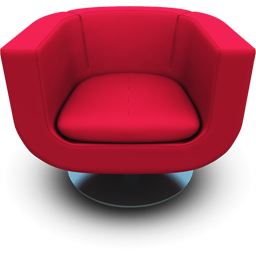
\includegraphics[width=0.19\textwidth]{magenta}
    \end{center}
    \vspace{-40pt}
  \end{wrapfigure}

  \section{Yard}

  YARD is a documentation generation tool for the Ruby programming language. It enables 
  the user to generate consistent, usable documentation that can be exported to a number 
  of formats very easily, and also supports extending for custom Ruby constructs such 
  as custom class level definitions. Above is a highlight of the some of YARD's notable features.

   Update the rake and guard file.

  \begin{lstlisting}
     $ vim Gemfile
     gem "yard"
     $ bundle
     $ yardoc # to generate new documentation
     $ vim Rakefile
     require 'rdoc/task'
     ...
     YARD::Rake::YardocTask.new
     ...
     $ vim Guardfile

     guard rake, :task => 'yard' do                                                
       watch(%r{^lib/(.+)\.rb)                                                       
       watch(%r{^(markdown|md|rdoc|)})                                               
      end                                                                             

    \end{lstlisting}

   \begin{lstlisting}
   # @author Yakuda Katz 
   # @return [String] description
   # @param name [Conway::Cell] description 
   # @param name [#method] description 
   ...
   # @see Conway::World 
   # @see Conway::World#method
   # @see #method 
   ...
   # @example descrprion
   #   Cell.new(state: :dead),alive? #false
   ...
   # @yield [ cell ] cell description
   # @yieldparam cell [Conway::Cell] description
   # @note description
   ...
   # @!group Name
    ...
   # @!endgroup 
   # only first word count rest is show as descripiton 
   # ... {Word#method descripiton} ... 
   # {link text}
   # {include:file:config/example.rdoc}
   # {include:Conway::Utils::Serializer} # show the comment
   \end{lstlisting}

   Here you can see an example of generated documentation 
   \href{http://www.rubydoc.info/gems/yard/index}{Yardoc}.

 \section{Conclussion}

    After analyzing the avalaible tools for generation documentation of your code
    I found out that most of them support additional features that will help to easily 
    browse and read the existing code. You can add comments to your code using markdown
    syntax thus when the documentation will be generated it will be outputed in the format you
    desire. Most of these tool provide a lot functionality out of the box and provide an easy way
    to create documentation for your code.

\end{document}

